\documentclass{article}

\usepackage{afterpage}
\usepackage{fontspec}
\usepackage{geometry}
\usepackage{hyperref}
\usepackage{lscape}
\usepackage{siunitx}
\usepackage{titling}

\newcommand*{\subtitle}[1]{\gdef\thesubtitle{#1}}

\title{CRAPS Kernel}
\subtitle{Software Development Plan}
\author{
       Maxime Arthaud
  \and Korantin Auguste
  \and Martin Carton
  \and Étienne Lebrun
}

\newcommand{\risk}[4]{%
  \noindent
  \begin{center}
    \begin{tabular}{|p{0.8\textwidth}|c|}
        \hline
        #2 & $#1$
      \\\hline
        \multicolumn{2}{|p{0.9\textwidth}|}{#3}
      \\\hline
        \multicolumn{2}{|p{0.9\textwidth}|}{#4}
      \\\hline
    \end{tabular}
  \end{center}
}

\begin{document}
  \begin{titlepage}
  \begin{center}
    
\includegraphics[height=1cm]{LogoEnseeiht}\\\vspace{1cm}
    \hrule\vspace{0.5cm}
    \textsc{\Large\thesubtitle}
    \\\vspace{0.5cm}

    \textbf{\huge\thetitle}
    \\\vspace{0.4cm}
    \hrule\vspace{2cm}

    {\large
      Maxime~\textsc{Arthaud}      \\
      Korantin~\textsc{Auguste}    \\
      Martin~\textsc{Carton}       \\
      Étienne~\textsc{Lebrun}
    }

    \vfill
    {\large January -- March 2015}
  \end{center}
\end{titlepage}

  \tableofcontents
  \newpage

  \section{Introduction}
    This project, suggested by Daniel Hagimont, is based on the CRAPS processor
    developed by Jean-Christophe Buisson and used in the first-year CPU
    architecture courses at ENSEEIHT. The goal is to develop an operating
    system that would run on top of that processor.

    The reasons for that project are that before, it was only possible to do a
    little of assembly directly on the processor to see it work, but nothing
    more.  After our project, it should be possible for students to really see
    the layer that goes on top of the CPU in modern computers: the operating
    system. So that the students can really make the link between the processor
    they just built and the computer and underlying operating systems they use
    everyday.

    \paragraph{}
    The system will be as modular as possible, so that students can reuse parts
    of it and implement their own modules.

    \begin{figure}[h]
      \centering
      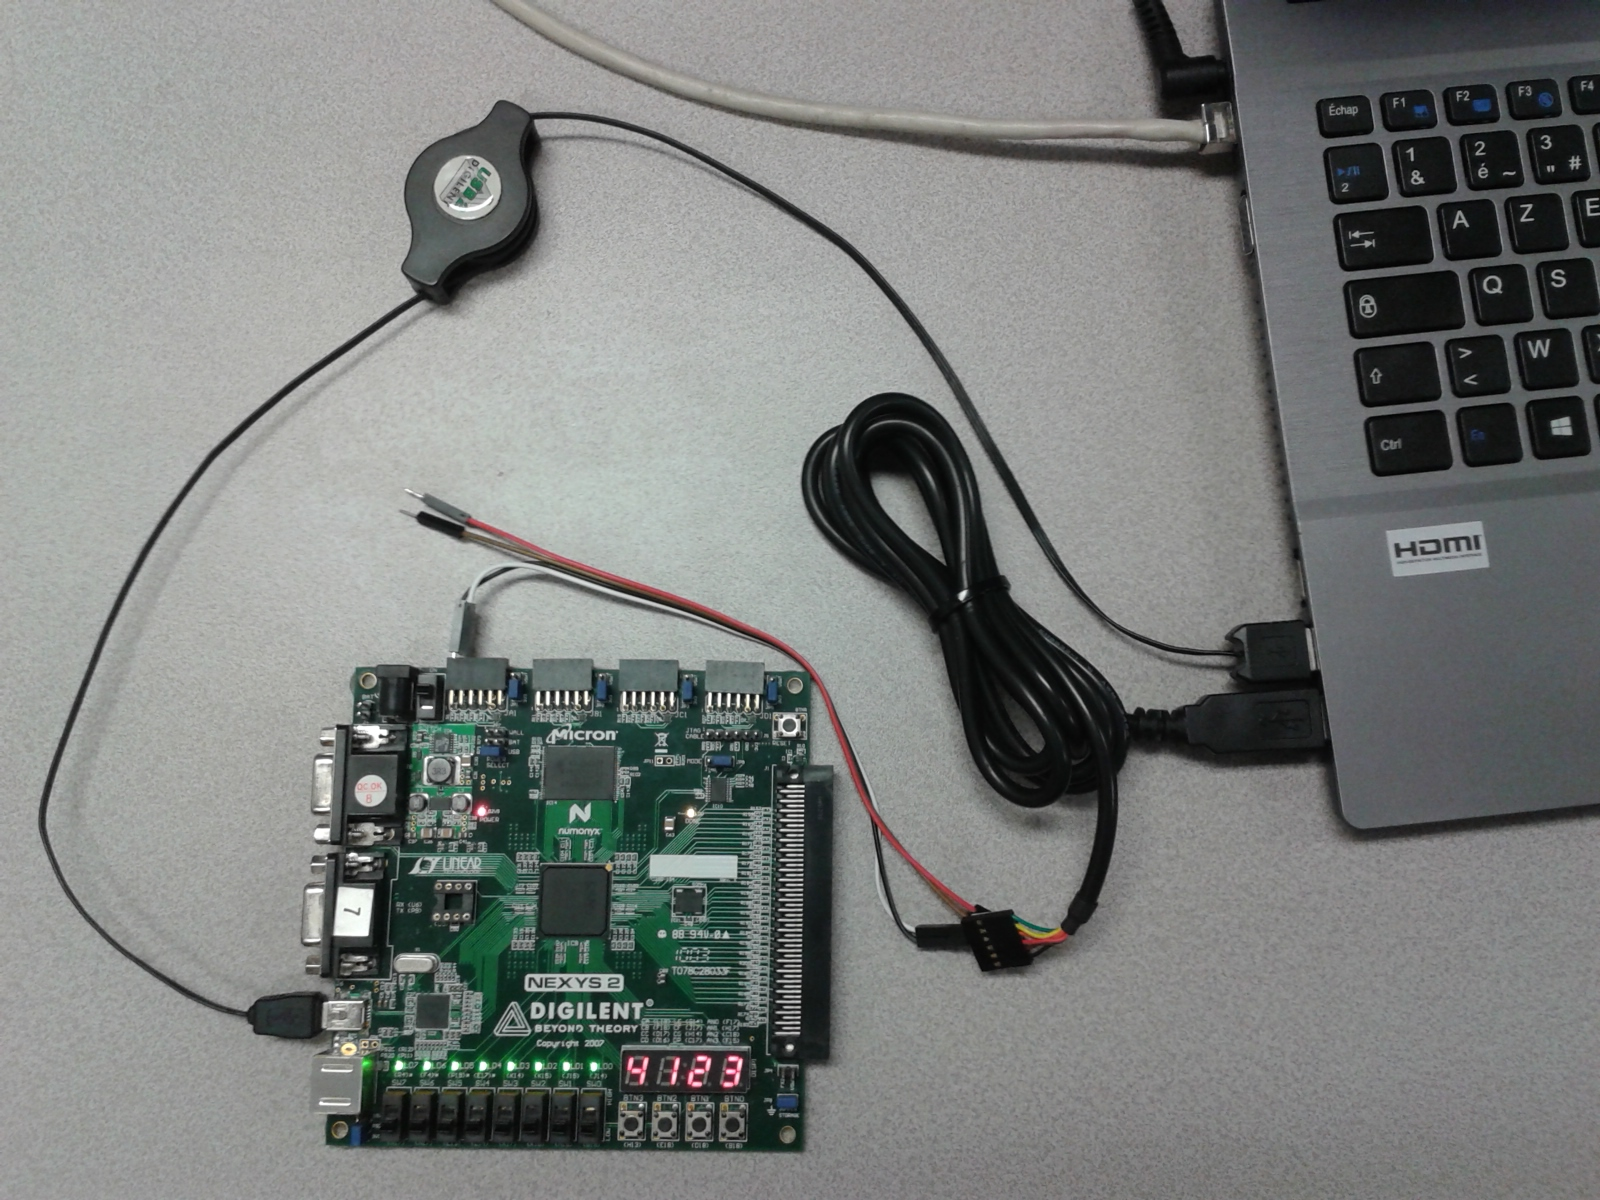
\includegraphics[width=0.8\textwidth]{./fig/Nexys2.jpg}
      \caption{A Nexys2 board}
    \end{figure}

  \section{Project Overview}
    The objective of the project is to create an operating system, with a
    scheduler running a few tasks. It will also provide functions to display
    text to the user, do input/output to a permanent storage\dots

    For now, having the OS loading programs dynamically is out-of-scope: the
    goal is to have a very simple functional OS.  We will also have to improve
    the CPU to make it support our OS. Specifically we know we will have to
    support the RAM chips that are on the FPGA: currently, we have \SI{2}{kB}
    of RAM that are built in, but that's clearly not enough.

    We will also need to adapt the tools that have been developed for the
    original craps. Some aspects of the tools need to be reworked. For
    instance, the additional RAM is not displayed. They are also working only on
    Microsoft Windows, and we would also like to have them work on GNU/Linux
    systems.

    Another important and time-consuming element will be to adapt the C compiler
    we made last year during a project, to make it generate the CRAPS assembly
    instead of x86 assembly.

  \section{Method, Tools and Test Facilities}
    \subsection{Method and Tools}
    A room and two FPGAs have been made available for us to work.
    The operating system will be written in C once we have a functional
    compiler.
    At the end, we want to be able to run a few processes that will communicate
    with the user, and store data in permanent memory.

     \subsection{Test Facilities}
    Tests are quite a though point, as our only way to test is to put
    our code on the board and try it. With the given software, it can not be
    done automatically.
    We will explore the feasibility to rewrite the monitor to be able to load
    the assembly code with a command line, which would allow automatization, but
    it could take too much time.
    We will produce test code for the functionalities we choose to implement.

  \section{Software Team Organisation and Responsibilities}
    \begin{itemize}
      \item Korantin Auguste as \textit{developer}
      \item Maxime Arthaud as \textit{tester}
      \item Martin Carton as \textit{project leader}
      \item Étienne Lebrun as \textit{quality manager}
    \end{itemize}

  \section{Meetings and Reporting}
    Two kinds of meetings are planned:
    \begin{itemize}
        \item a meeting once a week with the client;
        \item a meeting once a week with the industrial supervisor.
    \end{itemize}
    Minutes of these meetings are available is the repository.

    Additionally we regularly meet to talk about the advancement of the project.

  \section{Management of Actions}
    A file with the actions (listing who did what and when) has been created.

  \section{Management of Risks}
    For each risk, the product $\text{probability} \times \text{gravity}$ is
    shown in the top-right cell. If the product is above 6, the risk is
    considered critical.

    \risk{3 \times 3 = 9}{
      A FPGA can be damaged, making any test impossible.
    }{
      This is likely to happen and very problematic but we have two FPGAs and
      the possibility to have more in case of problem.
    }{
      Actually, we have 6 FPGAs, the risk is considered closed.
    }

    \risk{2 \times 3 = 6}{
      We may not be able to integrate the RAM, leading to huge memory
      limitations that may make the project impossible.
    }{
      We are now able to use the RAM, the risk is closed.
    }{
      In case of memory limitations, we can try to optimize the size of the code
      we generate.
    }

    \risk{3 \times 1 = 3}{
      The communication between the board and the computer might be too slow.
    }{
      We will have to be very careful to send just what is needed.
    }{
      We would need to limit the communication. It is not necessarily a problem
      as this is just to show students how to implement a simple communication
      protocol.
    }

  \section{Management of Change Requests}
    When a change request occurs from the client, we evaluate the additional
    time it may take, in order to decide whether it can be incorporated to the
    delivery and what would be the cost in terms of delay.

  \section{Quality and Configuration Management}
    We have decided to use a version control system to record every document and
    all the source code produced. A Git repository has been created on
    Github\footnote{Github repository:
    \url{https://github.com/mcarton/CRAPS-Kernel}}.
    It will contain:
    \begin{itemize}
      \item The source code of our project, for the processor as well as for the
            operating system
      \item The test code we produce according to the software test plan
      \item The documentation, as described in the following section
    \end{itemize}

    We impose some coding rules for what we do, but the project contains code
    from different preexisting projects with no common coding rules (if at all),
    so it is difficult to keep consistent.

  \section{Documentation}
    As the system will be modular and expected to be used by students, a
    documentation of every module will be provided.

    \begin{itemize}
      \item User Manual
      \item Modifications we did to the CRAPS processor
      \item This present Software Development Plan
      \item The specifications
      \item The test plan and test reports
    \end{itemize}

    \section{Deliveries}
      The software will be delivered in several iterations.
      Each delivery will be accompanied by the corresponding documentation.

      Delivery dates:
      \begin{description}
        \item[Version with basic functionalities] February 22
        \item[RS-232 Version] February 6
        \item[Version with persistent storage] If we have time ?
      \end{description}

    \newgeometry{top=1cm,bottom=1cm}
    \thispagestyle{empty}
    \begin{figure}
      \centering
      \includegraphics[
        angle=90,
        width=\linewidth,
        height=\textheight
      ]{Gantt.pdf}
      \label{fig:gantt}
    \end{figure}
    \clearpage
    \restoregeometry
\end{document}
